\section{Creearea unei aplicatii Android}
\subsection{Project template}
Sablonul pentru acest proiect poate fi descarcat de pe GitHub: \url{https://github.com/Dantsz/ProiectTWDM}
\subsubsection{Initializarea proiectului}
\begin{enumerate}
    \item clonati proiectul de pe GitHub
          \begin{lstlisting}
            git clone git@github.com:Dantsz/ProiectTWDM.git
        \end{lstlisting}
    \item deschideti Android Studio
    \item selectati \textit{Open}
    \item selectati directorul in care ati clonat proiectul
          \begin{figure}[H]
              \centering
              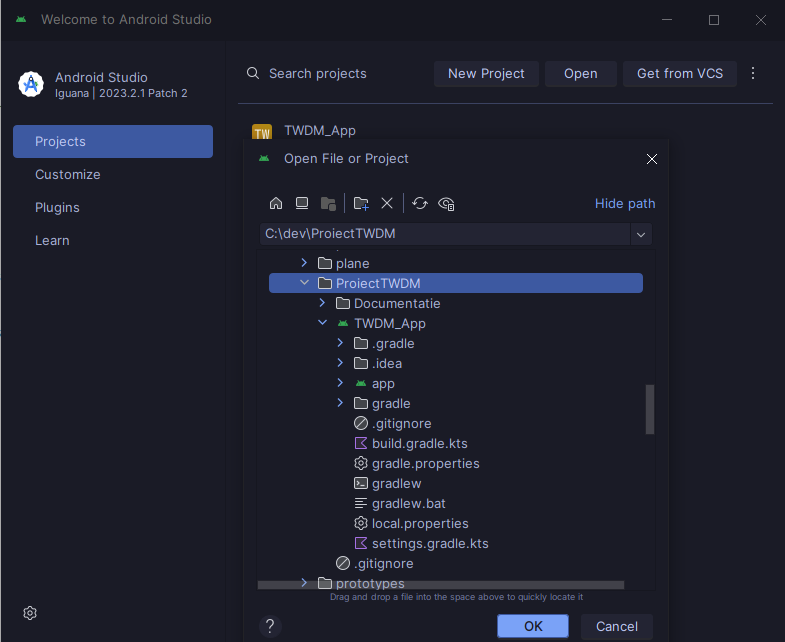
\includegraphics[width=0.7\linewidth]{figs/open_project.png}
              \caption{Deschiderea proiectului}
              \label{fig:open_project}
          \end{figure}
\end{enumerate}
\subsubsection{Structura proiectului}
Un proiect Android are o structura specifica, in care fisierele sunt organizate in directoare specifice.
\begin{itemize}
    \item \texttt{Fisierul manifest} descrie proprietati ale aplicatiei, cum ar fi permisiunile necesare.
    \item \texttt{Folderul kotlin + java} contine codul sursa al aplicatiei.
    \item \texttt{Folderul res} contine fisiere xml care descriu interfata grafica, imagini, string-uri si alte resurse.
\end{itemize}
\paragraph{Model View ViewModel}
Aplicatia foloseste arhitectura MVVM, care separa logica de afisare de logica de business.
\begin{figure}[H]
    \centering
    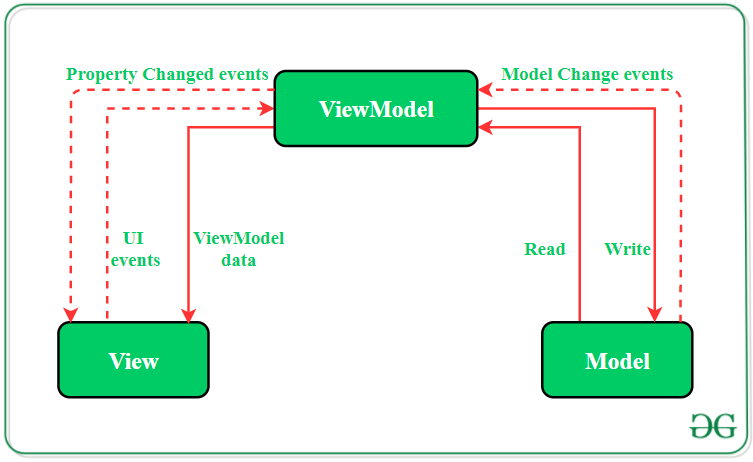
\includegraphics[width=0.7\linewidth]{figs/mvvm.png}
    \caption{Arhitectura MVVM}
    \label{fig:mvvm}
\end{figure}
In contextul acestei aplicatii fiecare fereastra are un ViewModel asociat, care defineste
datele si operatiile care pot fi efectuate pe aceste date.

\subsection{Rulare}
Pentru a rula aplicatia din Android Studio,
controalele implicite sunt: Shift + F10, sau folosind butonul de Run din bara de meniu de sus.
Pentru a selecta dizpovitivul pe care doriti sa rulati aplicatia, puteti folosi butonul de selectie a dispozitivului.
\begin{figure}[H]
    \centering
    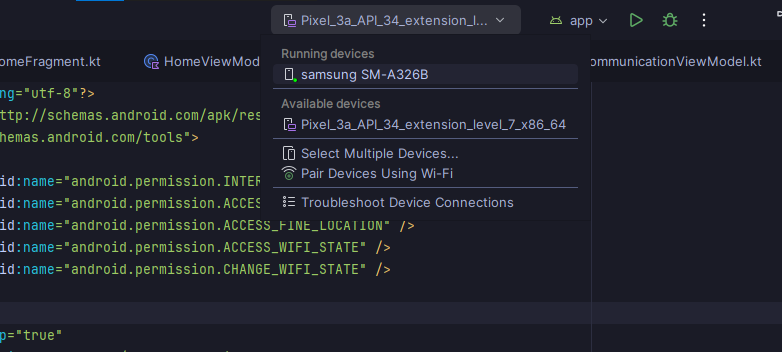
\includegraphics[width=0.7\linewidth]{figs/select_device.png}
    \caption{Selectarea dispozitivului}
    \label{fig:select_device}
\end{figure}